\section{Hardware development} \label{sec:hardware-devel}

% Motor Assembly
% `- Encoder soldering
% `- Cable soldering
% `- Magnetic disc attachment
\subsection{Motor assembly}
We began working on the hardware implementation by assembling the motor parts, which require some soldering.
First we soldered the encoder board on the motor terminals, being careful to leave enough motor shaft length available to be able to attach the encoder's magnetic disc on it.
Then we proceeded to solder a 6-wire cable to the encoder board terminals, which export all necessary electrical connections.
The exported connections are the encoder power supply ($VCC$ and $GND$, assigned to the blue/white-blue wire pair), the encoder output signals ($A$ and $B$, assigned to the green/white-green wire pair) and the motor power signals ($M1$ and $M2$, assigned to the orange/white-orange wire pair) and they can be visualized on \autoref{fig:encoder_board}.
Due to the development of the project having been done from home, for reasons of simplicity and availability of resources we used a generic 8-wire Ethernet UTP cable for the above mentioned electrical connections, as seen in \autoref{fig:motor_assembled}.
Finally we attached the magnetic disc on the motor shaft so the encoder can work as expected.

\begin{figure}[htp]
	\centering
	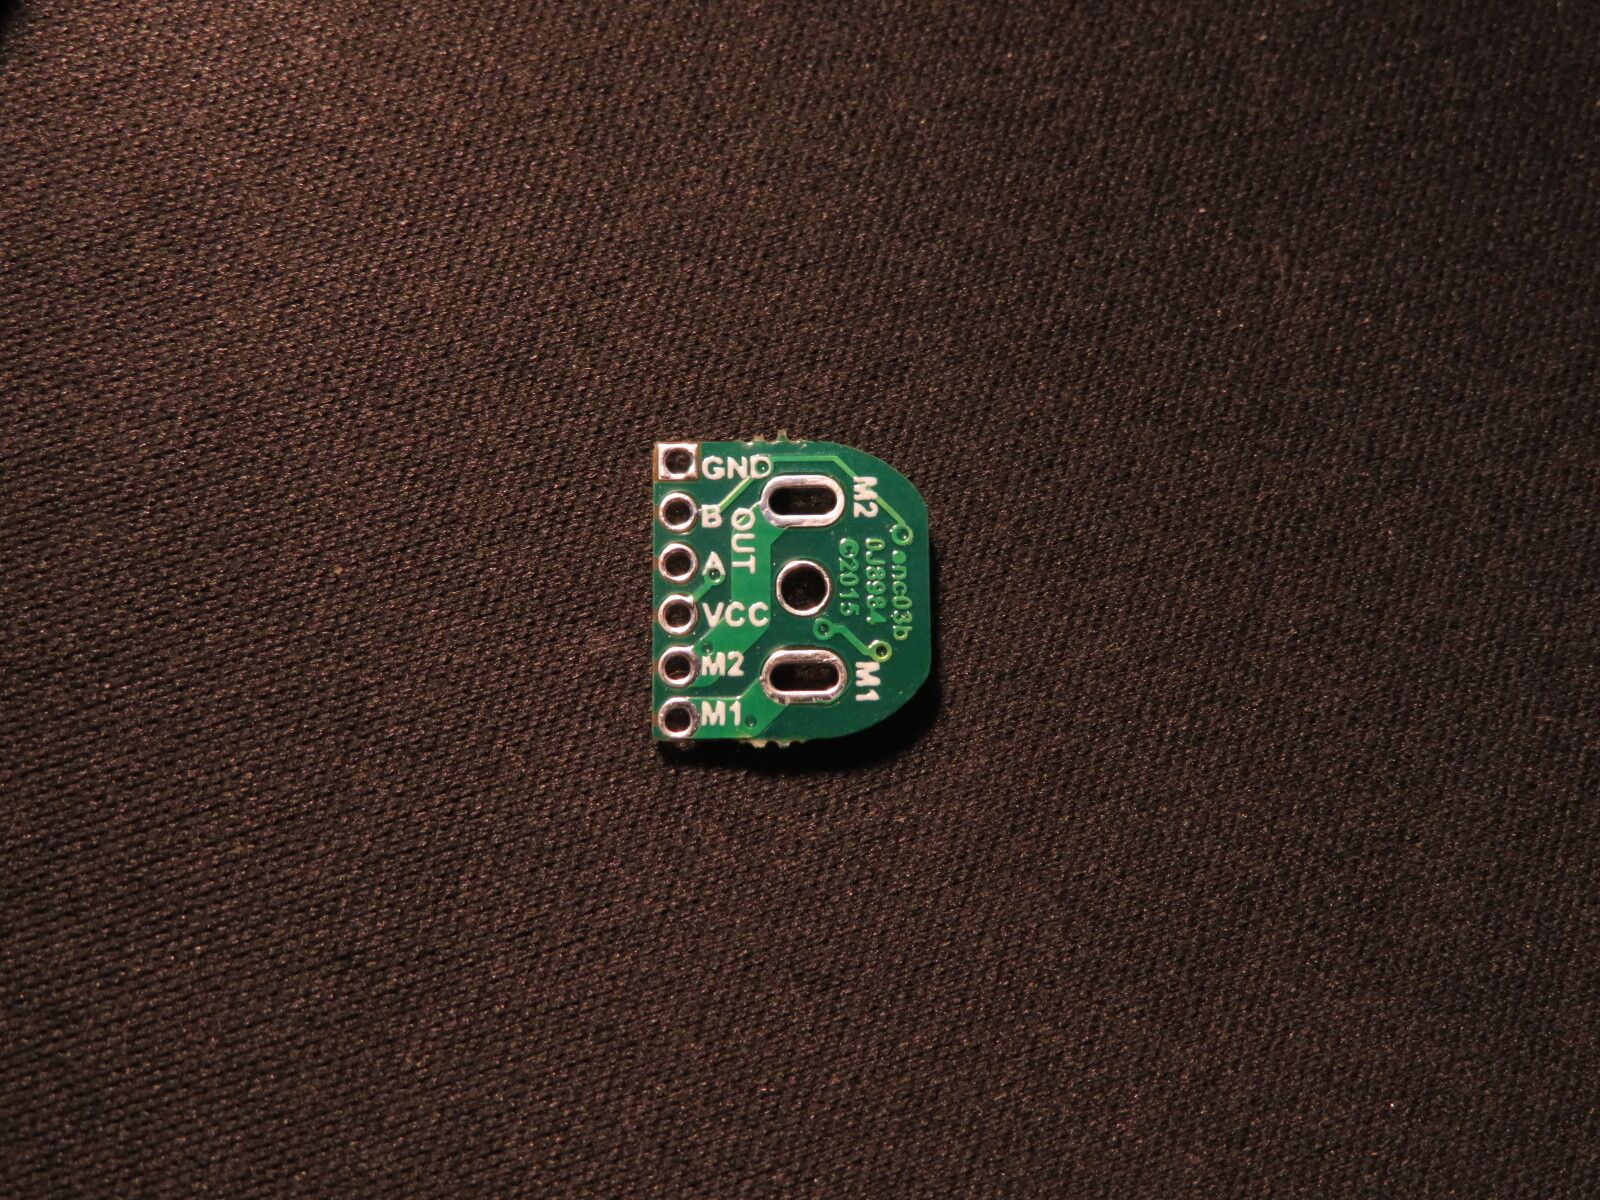
\includegraphics[width=0.8\textwidth]{IMG_2824_scaled.JPG}
	\caption{Motor encoder board connections}
	\label{fig:encoder_board}
\end{figure}

\begin{figure}[htp]
	\centering
	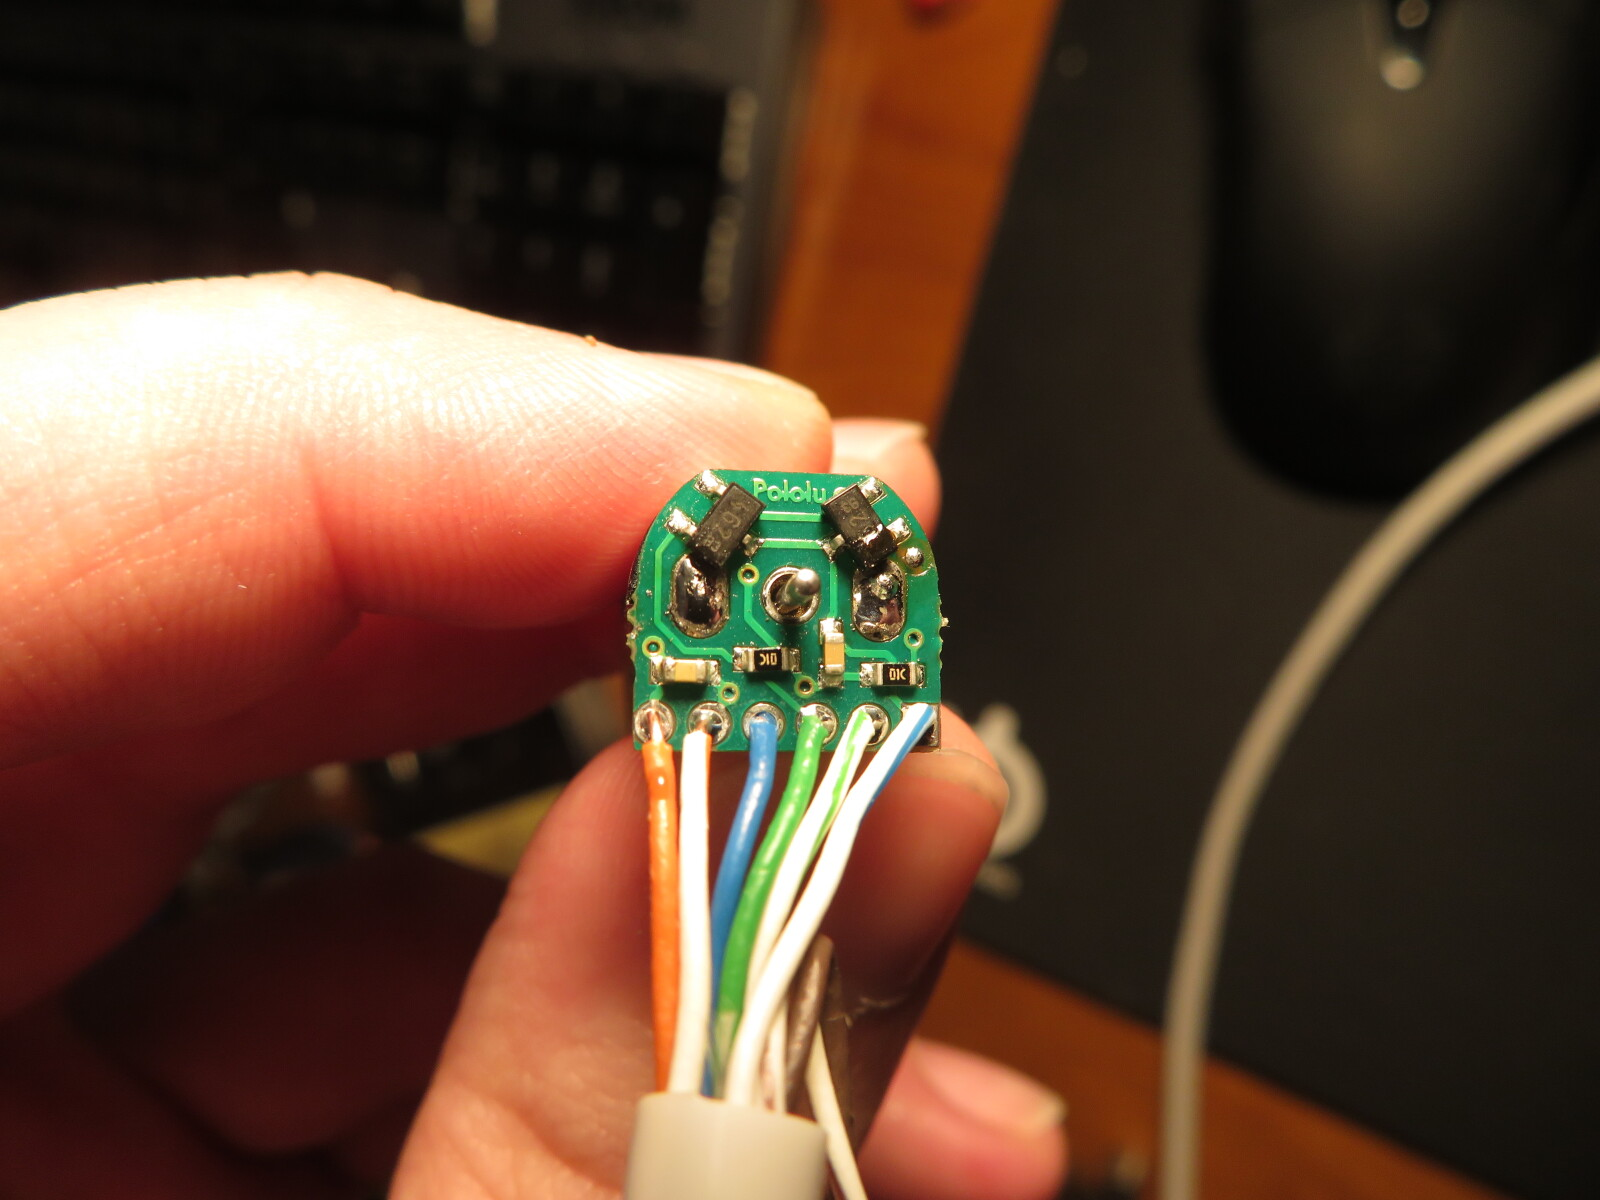
\includegraphics[width=0.8\textwidth]{IMG_2825_scaled.JPG}
	\caption{Encoder board and cables soldered to the motor}
	\label{fig:motor_assembled}
\end{figure}

% Motor Support
% `- 3D design
% `- 3D printing
% `- Adding the motor

% Raspberry Pi stack assembly
% `- Raspberry Pi
% `- GPIO exporter
%   `- encoder cables
% `- DFR0592
%   `- PSU cable
% `- netHAT 52-RTE
